\documentclass{article}

\usepackage[normalem]{ulem}
\usepackage{fancyhdr}
\usepackage[parfill]{parskip}
\usepackage{tikz}
\usepackage{multicol}
\pagestyle{fancyplain}

\title{Photosynthesis}
\author{Todd Davies}
\date{\today}

\begin{document}

\rhead{Photosynthesis}
\lhead{\today}

\maketitle

\section*{What is Photosynthesis?}
\thispagestyle{empty}
Photosynthesis is a metabolic reaction that takes place in plants and in some microorganims. The formulae for photosynthesis is:
\[
	6CO_2 + 6H_2O + energy \rightarrow C_6H_{12}O_6 + 6O_2
\]
The goal of photosynthesis is to use light energy (usually from the Sun) to turn carbon dioxide and water into sugars that the organism can use to respire. It is a reduction reaction since carbon dioxide and water are both reduced.

Photosynthesis takes place in the \textit{chloroplasts}.
\section*{ATP as an energy store}
Organisms use a molecule called ATP (adenosine triphosphate) to store small amounts of energy in usable, portable and accessible amounts. ATP is often referred to as the energy currency of cells. 

As the name suggests, an ATP molecule has three phosphate groups. A phosphate (pi) molecule is added to ADP to make ATP:
\[
	ADP + pi + energy \rightarrow ATP
\]

Reasons that the body uses ATP as it's energy currency include:
\begin{itemize}
	\item Each ATP molecule contains a useful amount of energy. As a comparison, one glucose molecule would probably contain too much energy for cell reactions and so energy would be wasted as heat.
	\item ATP can be broken down to ADP very quickly and so energy can be released for use immediately.
\end{itemize}

\section*{How does photosynthesis work?}
There are two stages in photosynthesis, the \textbf{light dependent reaction} and the \textbf{light independent reaction}. They happen simultaneously and don't directly require each other in order to work.

However, the light independent reaction does need products from the light dependent reaction in order to have the energy it needs to work.

Here is a diagram of the interconnection between the reactions:

\begin{center}
	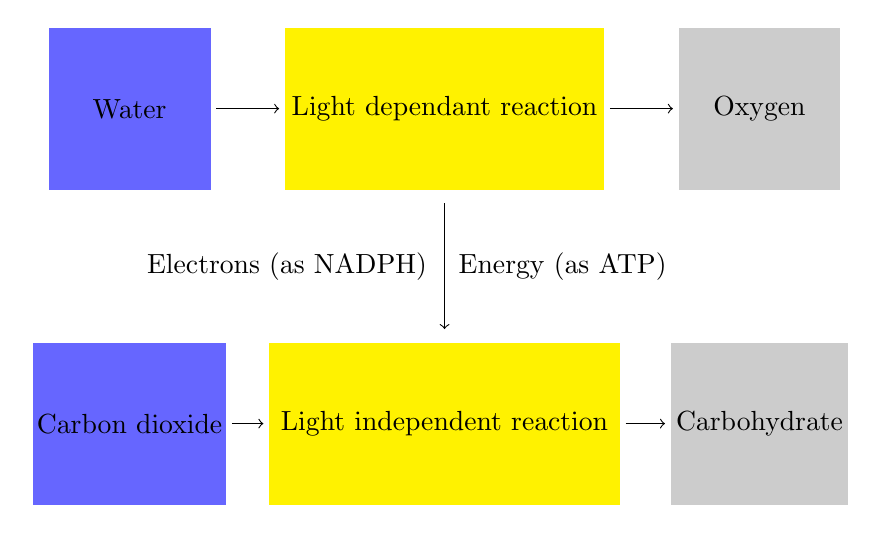
\begin{tikzpicture}
	%Top line
		%Water
		\draw [fill=blue!60,ultra thick,blue!60] (1, 1) rectangle (3, 3);
		\node at (2, 2) {Water};
		%Arrow to Light dependent reaction
		\draw [->] (3.1, 2) -- (3.9, 2);
		%Light dependent reaction
		\draw [fill=yellow,ultra thick,yellow] (4,  1) rectangle (8, 3);
		\node at (6, 2) {Light dependant reaction};
		%Arrow to Oxygen
		\draw [->] (8.1, 2) -- (8.9, 2);
		%Oxygen
		\draw [fill=black!20,ultra thick,black!20] (9, 1) rectangle (11, 3);
		\node at (10, 2) {Oxygen};
	%Bottom line
		%Carbon dioxide
		\draw [fill=blue!60,ultra thick,blue!60] (0.8, -1) rectangle (3.2, -3);
		\node at (2, -2) {Carbon dioxide};
		%Arrow to Light dependent reaction
		\draw [->] (3.3, -2) -- (3.7, -2);
		%Light dependent reaction
		\draw [fill=yellow,ultra thick,yellow] (3.8, -1) rectangle (8.2, -3);
		\node at (6, -2) {Light independent reaction};
		%Arrow to Oxygen
		\draw [->] (8.3, -2) -- (8.8, -2);
		%Oxygen
		\draw [fill=black!20,ultra thick,black!20] (8.9, -1) rectangle (11.1, -3);
		\node at (10, -2) {Carbohydrate};
	%Middle arrow
		\draw [->] (6, 0.8) -- (6, -0.8);
	%Middle labels
		\node at (4, 0) {Electrons (as NADPH)};
		\node at (7.5, 0) {Energy (as ATP)};
	\end{tikzpicture}
\end{center}

\subsection*{The light dependent reaction}
In this reaction, energy is captured from light by pigments such as chlorophyll and used to split water and create both ATP and NADP.

The light dependent reaction takes place in the \textbf{thylakoids}. The thylakoids contain pigments such as chlorophyll and other carotenoids. These molecules are able to absorb light and use it to boost an electron to higher energy levels. The energy from this electron is then used to power three different reactions:
\begin {itemize}
 \item Photolysis
 \item Photophosphorylation
 \item Production of reduced NADP
\end{itemize}

\newpage

\subsubsection*{Photolysis}
Here, the excited electrons from the chlorophyll are used to split water into three different parts:
\begin{itemize}
	\item Protons ($H^{+}$)
	\item Electrons ($e^{-}$)
	\item Oxygen
\end{itemize}
This is the reaction that produces the oxygen that is released into the environment. The equation for the reaction is as follows:
\[
	2H_2O \rightarrow 4H^+ + 4e^- + O_2
\]

\subsubsection*{Photophosphorylation}
The excited electrons are also used to produce ATP. The reaction is as follows:
\[
	ADP + Pi + \textrm{\textit{energy from excited electrons}} \rightarrow ATP
\]
This process is facilitated by many different electron carriers in the \textbf{electron transport chain}. The electron transport chain pumps hydrogen ions against their concentration gradient into spaces in the thylakoid membranes. The membrane is not permeable to hydrogen ions and so in order to flow back to the other side they must pass through ATPases which add a phosphate group to ADP molecules to create ATP.

\subsubsection*{Production of reduced NADP}
Since electrons can't react with most molecules on their own, they require an electron carrier such as NADP to facilitate transport and reactions. In order to retain it's neutral charge, NADP molecules accept both a proton and an electron when they are reduced.
\[
	NADP + H^+ + e^- +\textrm{\textit{energy from excited electrons}}\rightarrow \textrm{\textit{reduced NADP}}
\]

\subsubsection*{Key points:}
\begin{multicols}{2}
\begin{itemize}
    \item Takes place in thylakoids
    \item Electrons in chlorophyll excited
    \item Electrons in photolysis of water
    \item NADP is then reduced
    \item ATP generated from photophosphorylation
		\item ATPase acts as $H^+$ carrier
\end{itemize}
\end{multicols}

\subsection*{The light independent reaction}
The light dependent reaction takes place in the \textbf{stroma}. As the name suggests, this reaction doesn't need light to take place, however in practice this reaction does stop after dark since it requires resources from the light dependent reaction to function. In this stage of photosynthesis, carbon dioxide is taken from the atmosphere and turned into carbohydrates.

The Calvin cycle describes what happens during the light independent reaction:\\
\begin{center}
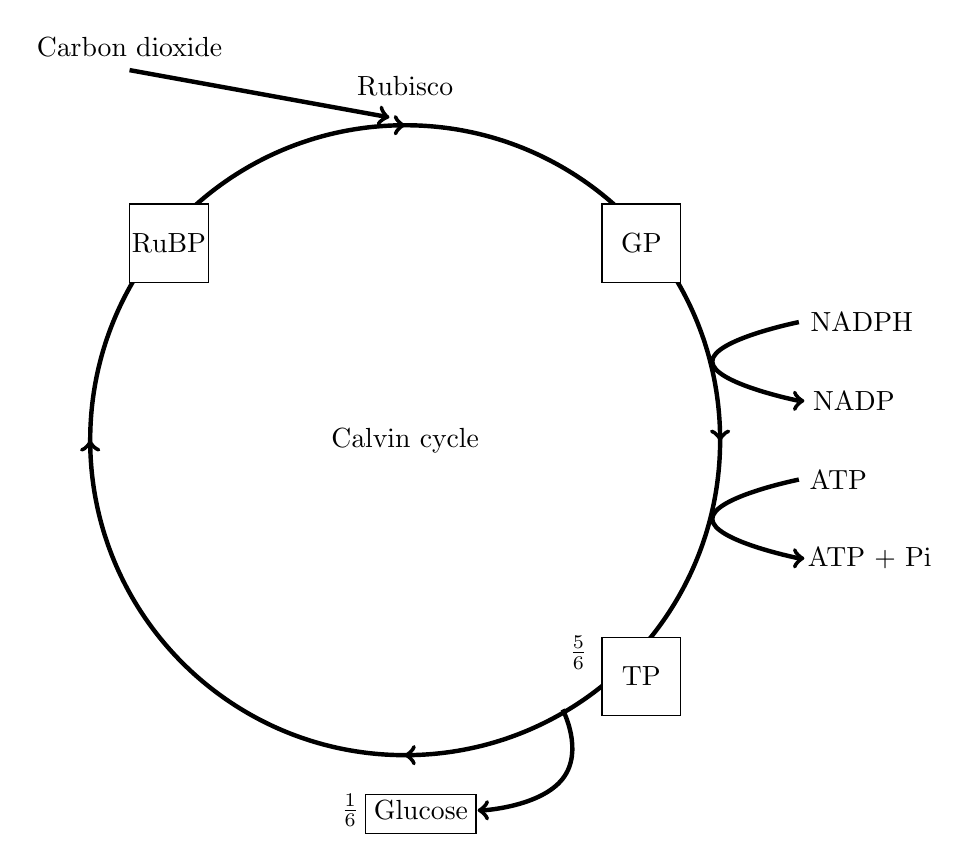
\begin{tikzpicture}
  %\draw[style=help lines] (-4, -4) grid[step=1cm] (8, 8);
	\draw [black, ultra thick] (2, 2) circle [radius=4];
	\node at (2, 2) {Calvin cycle};
	%Arrows around the circle
	\draw [ultra thick, ->] (2, -2) -- (1.99, -2); %Bottom
	\draw [ultra thick, ->] (1.99, 6) -- (2, 6);   %Top
	\draw [ultra thick, ->] (6, 2) -- (6, 1.99);   %Right
	\draw [ultra thick, ->] (-2, 1.99) -- (-2, 2); %Left
	%Carbon dioxide
	\node at (-1.5, 7) {Carbon dioxide};
	\draw [ultra thick, ->] (-1.5, 6.7) -- (1.8, 6.1);
	%Rubisco
	\node at (2, 6.5) {Rubisco};
	%GP
	\draw [fill=white] (5.5, 5) rectangle (4.5, 4);
	\node at (5, 4.5) {GP};
	%NADPH -> NADP
	\draw[ultra thick] plot [smooth,tension=1] coordinates{(7, 3.5) (5.9, 3) (7, 2.5)};
	\draw [ultra thick, ->] (7, 2.5) -- (7.07, 2.5);   %Right
	\node at (7.8, 3.5) {NADPH};
	\node at (7.7, 2.5) {NADP};
	%ATP -> ATP + Pi
	\draw[ultra thick] plot [smooth,tension=1] coordinates{(7, 1.5) (5.9, 1) (7, 0.5)};
	\draw [ultra thick, ->] (7, 0.5) -- (7.07, 0.5);   %Right
	\node at (7.5, 1.5) {ATP};
	\node at (7.9, 0.5) {ATP + Pi};
	%TP
	\draw [fill=white] (5.5, -0.5) rectangle (4.5, -1.5);
	\node at (5, -1) {TP};
	\node at (4.2, -0.7) {$\frac{5}{6}$};
	%RuBP
	\draw [fill=white] (-1.5, 5) rectangle (-0.5, 4);
	\node at (-1, 4.5) {RuBP};
	%TP -> Glucose
	\draw[ultra thick] plot [smooth,tension=1] coordinates{(4, -1.42) (4, -2.3) (3, -2.7)};
	\draw [ultra thick, ->] (3, -2.7)-- (2.92, -2.7);
	%Glucose
	\draw [fill=white] (1.5, -2.5) rectangle (2.9, -3);
	\node at (2.2, -2.7) {Glucose};
	\node at (1.3, -2.7) {$\frac{1}{6}$};
\end{tikzpicture}
\end{center}

In the cycle, Carbon dioxide is first combined with RuBP (catalysed by the enzyme Rubisco). The product if this reaction is two GP molecules. The carbon dioxide is now said to be fixed. Energy from ATP and electrons from NADPH are used to reduce the GP into TP, a three carbon sugar. Most of the TP ($\frac{5}{6}$) is used to form RuBP again, but the rest ($\frac{1}{6}$) is used to form Glucose. TP is quite a useful compound, it can be converted to lipids, proteins, larger sugars, starch etc.
\newpage
All these compounds are a lot to remember, here's a table illustrating them:
\begin{center}
	\begin{tabular}{|l|l|l|}
		\hline
			Name & \# Carbon atoms & Type\\ \hline
			Carbon dioxide & 1 & Inorganic\\ \hline
			Rubisco & N/A & Enzyme\\ \hline
			GP & 3 & Organic - not a carbohydrate\\ \hline
			TP & 3 & Organic - 3 carbon sugar\\ \hline
			Glucose & 6 & Organic - 6 carbon sugar\\ \hline
			RuBP & 5 & Organic\\ \hline
	\end{tabular}
\end{center}


\section*{Limiting factors}
\subsection*{Light}
\begin{itemize}
	\item Light with unsuitable wavelengths may not be suitable for photosynthesis.
	\item If there is light for a short period of time, the plant won't photosynthesise very much.
	\item Light of low intensity is a limiting factor (rate of photosynthesis usually increases proportionally to intensity if the limiting factor is intensity).
\end{itemize}
If the light intensity is the limiting factor, and the light intensity increases, then the rate of photosynthesis doesn't increase forever. There is a point where either the plant cannot physically photosynthesise any faster or another factor will become limiting (such as $CO_2$) concentration.

Very high light intensities may damage the plant and reduce photosynthesis.

\subsection*{Temperature}
Temperature doesn't have an effect on the light dependent reaction, since this reaction is powered by light, not kinetic energy. However, the light independent reaction is reliant upon collisions between molecules and is therefore affected by temperature.

Very high temperatures will denature enzymes and slow photosynthesis.

\subsection*{Carbon dioxide concentration}
In areas of high fauna density, carbon dioxide can be a precious resource and becomes a limiting factor. Since in normal air, $CO_2$ concentration is around 0.04\%, the limiting factor for most crops is the concentration of carbon dioxide.


\section*{Managing greenhouses}
Greenhouses are ideal environments for examiners to use in questions about photosynthesis. With proper management, they can produce higher yields, grow unusual crops and grow crops out of season. They can do this by controlling conditions that are the limiting factors of plants.

Greenhouses can have automatic sprinkler systems and humidifiers to keep the water levels correct, paraffin heaters to supply $CO_2$ and keep the temperature just right and artificial lighting to keep photosynthesis going throughout the night. These systems can be controlled by computers that will constantly monitor the conditions and keep them optimum.

However, greenhouse owners must be careful not to spend too much money increasing the yield of their crops, the cost of the heating, computer systems and light etc may outweigh the extra money gained from the high yield.


\section*{Questions to practice}
\subsection*{Question 1}
Where does the light independent and the light dependent reactions take place?

\textbf{Answer}\\
The light independent reaction takes place in the stroma and the light dependent reaction takes place in the thylakoid membrane.

\subsection*{Question 2}
Give an example of oxidation in the Calvin cycle.

\textbf{Answer}\\
Reduced NADP is oxidised to NADP.

\subsection*{Question 3}
How is the structure of the chloroplast adapted for it's function?

\textbf{Answer}\\
The thylakoid membrane has a large surface area, and since it contains the chlorophyll, this means that large amounts of light can be absorbed.

The stroma has a membrane around it which prevents the light independent reaction from mixing with the cytoplasm. This is advantageous since it means the enzymes in the light independent reaction are at a high concentration here and so the reaction is faster.

\subsection*{Question 4}
Explain why chlorophyll is green.

\textbf{Answer}\\
Chlorophyll doesn't absorb light with wavelengths that correspond to green light and so these photons are reflected making it appear green.

\subsection*{Question 5}
Why is it advantageous for plants to have other light absorbing pigments as well as chlorophyll?

\textbf{Answer}\\
Having several different pigments allows plants to absorb a greater range of wavelengths of light and so increase the efficiency of photosynthesis. Some pigments may absorb light that would damage other pigments and so the other pigments are protected.
\end{document}